\documentclass[a4paper]{article}
\usepackage{enumitem, amsmath, gensymb, graphicx, caption, amssymb, geometry, fancyhdr, arydshln, adjustbox,float}

\geometry{left=1in, right=1in, top=1in, bottom=1in}
\pagestyle{fancy}

\newcommand{\myName}{\textbf{Shantanu Ghodgaonkar}\\\textit{Univ ID}: N11344563\\\textit{Net ID}: sng8399\\\textit{Ph.No.}: +1 (929) 922-0614}
\newlist{qalist}{description}{1}
\setlist[qalist]{style=unboxed,leftmargin=0.5cm,labelwidth=2.5cm}


\title{Homework 4 Answers : ROB-GY 6103}
\author{\myName}
\date{\today}

\fancyhead{} % Clear existing header settings 
\fancyhead[L]{\today}
\fancyhead[R]{N11344563}


\begin{document}
	
	\begin{titlepage}
	    \centering
	    \vspace{2cm}
	    \Huge\textbf{Mathematics for Robotics \\ ROB-GY 6103 \\ Homework 4 Answers}
	    \vspace{1cm}
	    \\ \Large \today
	    \vfill
	    \Large \myName
	\end{titlepage}
	
	\begin{qalist}			
		\item[Question: 1.] \setcounter{equation}{0}
		\item[Answer:] Firstly, consider the inner product $\langle x,y \rangle = {x}^{T}\bar{y}$. To show that it is an inner product over $({\mathbb{C}}^{n}, \mathbb{C})$ we need to check if it follow the following properties - 
		\begin{enumerate}[label=\alph*., align=left]
			\item $\langle x,y \rangle = \overline{\langle y,x \rangle}$
				\begin{equation}\label{eq:q11alhs}
					LHS = \langle x,y \rangle = {x}^{T}\bar{y}
				\end{equation}
				Let $x = \begin{bmatrix}{x}_{1} \\ {x}_{2}\end{bmatrix}$ and $y = \begin{bmatrix}{y}_{1} \\ {y}_{2}\end{bmatrix}$. Substituting in ${Eq}^{n}(\ref{eq:q11alhs}) \Rightarrow$
				\begin{equation}
					LHS = \begin{bmatrix}{x}_{1} & {x}_{2}\end{bmatrix} \begin{bmatrix}\bar{{y}_{1}} \\ \bar{{y}_{2}}\end{bmatrix} = {x}_{1}\bar{{y}_{1}} + {x}_{2}\bar{{y}_{2}}
				\end{equation}
				Now consider, 
				\begin{equation}\label{eq:q11arhs}
					RHS = \overline{\langle x,y \rangle} = {y}^{T}\bar{x}
				\end{equation}
				Substituting the values for $x$ and $y$ in above ${Eq}^{n}(\ref{eq:q11arhs}) \Rightarrow$
				\begin{equation}
					RHS = \overline{\begin{bmatrix}{y}_{1} & {y}_{2}\end{bmatrix} \begin{bmatrix}\bar{{x}_{1}} \\ \bar{{x}_{2}}\end{bmatrix}} = \overline{{y}_{1}\bar{{x}_{1}} + {y}_{2}\bar{{x}_{2}}} = {x}_{1}\bar{{y}_{1}} + {x}_{2}\bar{{y}_{2}} = LHS
				\end{equation}
				
			\item $\langle {a}_{1}{x}_{1} + {a}_{2}{x}_{2},y \rangle = {a}_{1}\langle {x}_{1}, y \rangle + {a}_{2}\langle {x}_{2}, y \rangle$
				Let, ${x}_{1} = \begin{bmatrix}{x}_{11} \\ {x}_{12}\end{bmatrix}$, ${x}_{2} = \begin{bmatrix}{x}_{21} \\ {x}_{22}\end{bmatrix}$ and  $y = \begin{bmatrix}{y}_{1} \\ {y}_{2}\end{bmatrix}$. So, 
				\begin{align}
					\langle {a}_{1}{x}_{1} + {a}_{2}{x}_{2},y \rangle &= {({a}_{1}{x}_{1} + {a}_{2}{x}_{2})}^{T}\bar{y} \\
					%{({a}_{1}{x}_{1} + {a}_{2}{x}_{2})}^{T}\bar{y} 
					&= {\left[{a}_{1}\begin{bmatrix}{x}_{11} \\ {x}_{12}\end{bmatrix} +  {a}_{2}\begin{bmatrix}{x}_{21} \\ {x}_{22}\end{bmatrix}\right]}^{T}\begin{bmatrix}\bar{{y}_{1}} \\ \bar{{y}_{2}}\end{bmatrix} \\
					&= \begin{bmatrix}{a}_{1}{x}_{11}+{a}_{2}{x}_{21} & {a}_{1}{x}_{12}+{a}_{2}{x}_{22}\end{bmatrix} \begin{bmatrix}\bar{{y}_{1}} \\ \bar{{y}_{2}}\end{bmatrix} \\
					&= ({a}_{1}{x}_{11}+{a}_{2}{x}_{21})\bar{{y}_{1}} +  ({a}_{1}{x}_{12}+{a}_{2}{x}_{22})\bar{{y}_{2}} \\
					&= {a}_{1}{x}_{11}\bar{{y}_{1}} + {a}_{2}{x}_{21}\bar{{y}_{1}} + {a}_{1}{x}_{12}\bar{{y}_{2}} + {a}_{2}{x}_{22}\bar{{y}_{2}}\\
					&= {a}_{1}({x}_{11}\bar{{y}_{1}} + {x}_{12}\bar{{y}_{2}}) + {a}_{2}({x}_{21}\bar{{y}_{1}} + {x}_{22}\bar{{y}_{2}}) \\
					&= {a}_{1}\begin{bmatrix}{x}_{11} & {x}_{12}\end{bmatrix}\begin{bmatrix}\bar{{y}_{1}} \\ \bar{{y}_{2}}\end{bmatrix} + {a}_{2}\begin{bmatrix}{x}_{21} & {x}_{22}\end{bmatrix} \begin{bmatrix}\bar{{y}_{1}} \\ \bar{{y}_{2}}\end{bmatrix} \\
					&= {a}_{1}{{x}_{1}}^{T}\bar{y} + {a}_{2}{{x}_{2}}^{T}\bar{y} \\
					&= {a}_{1}\langle {x}_{1}, y \rangle + {a}_{2}\langle {x}_{2}, y \rangle
				\end{align} 
				
			\item $\langle x,x \rangle \;\geq 0 \text{ and } \langle x,x \rangle = 0 \Leftrightarrow x = 0$
				Let $x = \begin{bmatrix}{x}_{1} \\ {x}_{2}\end{bmatrix}$ s.t. ${x}_{1} = {a}_{1} + {b}_{1}\iota \text{ and } {x}_{2} = {a}_{2} + {b}_{2}\iota$ So, 
				\begin{align}
					\langle x,x \rangle &= \begin{bmatrix}{x}_{1} & {x}_{2}\end{bmatrix}\begin{bmatrix}\bar{{x}_{1}} \\ \bar{{x}_{2}}\end{bmatrix} \\
					&= {x}_{1}\bar{{x}_{1}} + {x}_{2}\bar{{x}_{2}} \\
					&= ({a}_{1} + {b}_{1}\iota)({a}_{1} - {b}_{1}\iota) + ({a}_{2} + {b}_{2}\iota)({a}_{2} - {b}_{2}\iota) \\ 
					&= ({{a}_{1}}^{2} + {{b}_{1}}^{2}) + ({{a}_{2}}^{2} + {{b}_{2}}^{2}) \label{eq:q11cFinal}
				\end{align}
				By observing above  ${Eq}^{n}(\ref{eq:q11cFinal})$ we can see that $\langle x,x \rangle$ will always be $\geq 0$ and \textit{iff} $x = 0 \Leftrightarrow \langle x,x \rangle = 0$.
		\end{enumerate}
		
		
		Secondly, consider the inner product $\langle x,y \rangle = {\bar{x}}^{T}y$. To show that it is an inner product over $({\mathbb{C}}^{n}, \mathbb{C})$ we need to check if it follow the following properties - 
		\begin{enumerate}[label=\alph*., align=left]
			\item $\langle x,y \rangle = \langle y,x \rangle$ for $\mathbb{F} = \mathbb{R}$. \\ \\
				Let $x = \begin{bmatrix}{x}_{1} \\ {x}_{2}\end{bmatrix}$ and $y = \begin{bmatrix}{y}_{1} \\ {y}_{2}\end{bmatrix}$. So,
				\begin{align}
					LHS &= \langle x,y \rangle = {\bar{x}}^{T}y \\
					&= \begin{bmatrix}\bar{{x}_{1}} & \bar{{x}_{2}}\end{bmatrix} \begin{bmatrix}{y}_{1} \\ {y}_{2}\end{bmatrix} \\
					&= \bar{{x}_{1}}{y}_{1} + \bar{{x}_{2}}{y}_{2} 
				\end{align}
				Assuming ${x}_{1}, {x}_{2}, {y}_{1} \text{ and } {y}_{2} \in \mathbb{R} \Rightarrow {x}_{1} = \bar{{x}_{1}},\;{x}_{2} = \bar{{x}_{2}},\;{y}_{1} = \bar{{y}_{1}},\; {y}_{2} = \bar{{y}_{2}}\Rightarrow$			
				\begin{align}
					&= {x}_{1}{y}_{1} + {x}_{2}{y}_{2} \\
					&= 2\bar{{y}_{1}}{x}_{1} + \bar{{y}_{2}}{x}_{2} \\
					&= \begin{bmatrix}\bar{{y}_{1}} & \bar{{y}_{2}}\end{bmatrix} \begin{bmatrix}{x}_{1} \\ {x}_{2}\end{bmatrix} \\
					&= \langle y,x \rangle
				\end{align}	
				
			\item $\langle x,y \rangle = \overline{\langle y,x \rangle}$ for $\mathbb{F} = \mathbb{C}$
				Let $x = \begin{bmatrix}{x}_{1} \\ {x}_{2}\end{bmatrix}$ and $y = \begin{bmatrix}{y}_{1} \\ {y}_{2}\end{bmatrix}$. So,
				\begin{align}
					\langle x,y \rangle &= {\bar{x}}^{T}y \\
					&= \begin{bmatrix}\bar{{x}_{1}} & \bar{{x}_{2}}\end{bmatrix} \begin{bmatrix}{y}_{1} \\ {y}_{2}\end{bmatrix} \\
					&= \bar{{x}_{1}}{y}_{1} + \bar{{x}_{2}}{y}_{2} \\
					&= \overline{\bar{{y}_{1}}{x}_{1} + \bar{{y}_{2}}{x}_{2}} \\
					&= \overline{\begin{bmatrix}\bar{{y}_{1}} & \bar{{y}_{2}}\end{bmatrix} \begin{bmatrix}{x}_{1} \\ {x}_{2}\end{bmatrix}} \\
					&= \overline{\langle y,x \rangle}
				\end{align}
				
			\item $\langle {a}_{1}{x}_{1} + {a}_{2}{x}_{2},y \rangle = {a}_{1}\langle {x}_{1}, y \rangle + {a}_{2}\langle {x}_{2}, y \rangle$ \\ \\
				Let, ${x}_{1} = \begin{bmatrix}{x}_{11} \\ {x}_{12}\end{bmatrix}$, ${x}_{2} = \begin{bmatrix}{x}_{21} \\ {x}_{22}\end{bmatrix}$ and  $y = \begin{bmatrix}{y}_{1} \\ {y}_{2}\end{bmatrix}$. So, 
				\begin{align}
					\langle {a}_{1}{x}_{1} + {a}_{2}{x}_{2},y \rangle &= {\overline{{a}_{1}{x}_{1} + {a}_{2}{x}_{2}}}^{T}y \\
					&= \begin{bmatrix}{a}_{1}\overline{{x}_{11}} + {a}_{2}\overline{{x}_{21}} & {a}_{1}\overline{{x}_{12}} + {a}_{2}\overline{{x}_{22}}\end{bmatrix} \begin{bmatrix}{y}_{1} \\ {y}_{2}\end{bmatrix}\\
					&= {a}_{1}\overline{{x}_{11}}{y}_{1} + {a}_{2}\overline{{x}_{21}}{y}_{1} + {a}_{1}\overline{{x}_{12}}{y}_{2} + {a}_{2}\overline{{x}_{22}}{y}_{2} \\
					&= {a}_{1}(\overline{{x}_{11}}{y}_{1} + \overline{{x}_{12}}{y}_{2}) + {a}_{2}(\overline{{x}_{21}}{y}_{1} + \overline{{x}_{22}}{y}_{2}) \\
					&= {a}_{1}{\bar{{x}_{1}}}^{T}y + {a}_{2}{\bar{{x}_{2}}}^{T}y \\
					&= {a}_{1}\langle {x}_{1}, y \rangle + {a}_{2}\langle {x}_{2}, y \rangle
				\end{align}
			\item $\langle x,x \rangle \;\geq 0 \text{ and } \langle x,x \rangle = 0 \Leftrightarrow x = 0$
				Let $x = \begin{bmatrix}{x}_{1} \\ {x}_{2}\end{bmatrix}$ s.t. ${x}_{1} = {a}_{1} + {b}_{1}\iota \text{ and } {x}_{2} = {a}_{2} + {b}_{2}\iota$ So, 
				\begin{align}
					\langle x,x \rangle &= {\bar{x}}^{T}x \\
					&= \begin{bmatrix}\bar{{x}_{1}} & \bar{{x}_{2}}\end{bmatrix}\begin{bmatrix}{x}_{1} \\ {x}_{2}\end{bmatrix}\\
					&= \bar{{x}_{1}}{x}_{1} + \bar{{x}_{2}}{x}_{2} \\
					&= ({a}_{1} + {b}_{1}\iota)({a}_{1} - {b}_{1}\iota) + ({a}_{2} + {b}_{2}\iota)({a}_{2} - {b}_{2}\iota) \\ 
					&= ({{a}_{1}}^{2} + {{b}_{1}}^{2}) + ({{a}_{2}}^{2} + {{b}_{2}}^{2}) \label{eq:q12cFinal}
				\end{align}
				By observing above  ${Eq}^{n}(\ref{eq:q12cFinal})$ we can see that $\langle x,x \rangle$ will always be $\geq 0$ and \textit{iff} $x = 0 \Leftrightarrow \langle x,x \rangle = 0$.
		\end{enumerate}
		
		\item[Question: 2.] \setcounter{equation}{0}
		\item[Answer:] We are given ${\mathbb{P}}_{3} ([-1,1])$ and the inner product $\langle p,q \rangle = {\int}_{-1}^{1} p(x)q(x)\;dx$. 
			It is also given that, 
			\begin{align}
				{p}_{0} &= 1 \\
				{p}_{1} &= x \\
				{p}_{2} &= \frac{3}{2}{x}^{2} - \frac{1}{2} \\
				{p}_{3} &= \frac{5}{2}{x}^{3} -\frac{3}{2}x
			\end{align}
			We can form the set $p = \{{p}_{0}, {p}_{1}, {p}_{2}, {p}_{3}\} = 
				\left\{\begin{bmatrix} 1 \\ 0 \\ 0 \\ 0 \end{bmatrix}
					 \begin{bmatrix} 0 \\ 1 \\ 0 \\ 0 \end{bmatrix}
					 \begin{bmatrix} -\frac{1}{2} \\ 0 \\ \frac{3}{2} \\ 0 \end{bmatrix}
					 \begin{bmatrix} 0 \\ -\frac{3}{2} \\ 0 \\ \frac{5}{2} \end{bmatrix}
				\right\}
				\text{First, we check for linear independance}\Rightarrow \begin{bmatrix}1 & 0 & -\frac{1}{2} & 0 \\ 0 & 1 & 0 & -\frac{3}{2} \\ 0 & 0 & \frac{3}{2} & 0 \\ 0 & 0 & 0 & \frac{3}{2}\end{bmatrix} \begin{bmatrix}{\alpha}_{1} \\ {\alpha}_{2} \\ {\alpha}_{3} \\ {\alpha}_{4}\end{bmatrix} = 0 \Rightarrow {\alpha}_{1} = {\alpha}_{2} = {\alpha}_{3} = {\alpha}_{4} = 0 \Rightarrow \text{the given set is \textit{Linearly Independant}.}$
			
			Now we shall check for orthogonality, as per the instruction given in the question $\rightarrow$
			\begin{align}
				\langle {p}_{0}, {p}_{3} \rangle &= {\int}_{-1}^{1} (1)\cdot\frac{5}{2}{x}^{3} -\frac{3}{2}x\;dx \\
				&= \left[ \frac{5}{8}{x}^{4} - \frac{3}{4}{x}^{2}\right]_{-1}^{1} \\
				&= \left(\frac{5}{8} - \frac{3}{4} \right) - \left(\frac{5}{8} - \frac{3}{4} \right) \\
				& = 0
			\end{align}
			\\
			\begin{align}
				\langle {p}_{1}, {p}_{2} \rangle &= {\int}_{-1}^{1} x \cdot \left(\frac{3}{2}{x}^{2} - \frac{1}{2}\right) \; dx \\
				&= {\int}_{-1}^{1}\frac{3}{2}{x}^{3} - \frac{1}{2}x\; dx \\
				&= \left[ \frac{3}{8}{x}^{4} - \frac{1}{4}{x}^{2}\right]_{-1}^{1} \\
				&= \left(\frac{3}{8} - \frac{1}{4} \right) - \left(\frac{3}{8} - \frac{1}{4} \right) \\
				& = 0
			\end{align}
			
			Hence, we can see that the set $p$ is \textit{Linearly Independant} and that its elements are orthogonal and it spans ${\mathbb{P}}_{3}$. 
			
			$\therefore \; p$ forms a orthogonal basis of ${\mathbb{P}}_{3}$.
			
			\textbf{Q.E.D.}
			
		\item[Question: 3.] \setcounter{equation}{0}
		\item[Answer:] Given the standard inner product $\langle x,y \rangle = {x}^{T}y$ and the vectors, 
			\begin{equation}
				{y}_{1} = \begin{bmatrix}1 \\ -2 \\ 1\end{bmatrix},\; {y}_{2} = \begin{bmatrix}4 \\ 0 \\ -1\end{bmatrix},\;{y}_{3} = \begin{bmatrix}-2 \\ 2 \\ 3\end{bmatrix}
			\end{equation}	
			We shall apply the Gram Schmidt Procedure to the given set of vectors. We know that, 
			\begin{equation}
				{v}_{k} = {y}_{k} - \sum_{j = 1}^{k-1} \frac{\langle {y}_{k}, {v}_{j}\rangle}{{||{v}_{j}||}^{2}} \cdot {v}_{j}
			\end{equation}
			
			So, \begin{align}
				{v}_{1} &= {y}_{1} = \begin{bmatrix}1 \\ -2 \\ 1\end{bmatrix} \\ \notag \\
				{v}_{2} &= {y}_{2} - \frac{\langle {y}_{2}, {v}_{1}\rangle}{{||{v}_{1}||}^{2}}  \cdot {v}_{1} \\
				\notag &= \begin{bmatrix}4 \\ 0 \\ -1\end{bmatrix} - \left( \frac{\begin{bmatrix}4 & 0 & -1\end{bmatrix} \begin{bmatrix}1 \\ -2 \\ 1\end{bmatrix}}{\begin{bmatrix}1 & -2 & 1\end{bmatrix}\begin{bmatrix}1 \\ -2 \\ 1\end{bmatrix}} \cdot \begin{bmatrix}1 \\ -2 \\ 1\end{bmatrix}\right) \\
				\notag &= \begin{bmatrix}4 \\ 0 \\ -1\end{bmatrix} - 0.5\cdot \begin{bmatrix}1 \\ -2 \\ 1\end{bmatrix} = \begin{bmatrix}3.5 \\ 1 \\ -1.5\end{bmatrix} \\ \notag \\
				{v}_{3} &= {y}_{3} - \frac{\langle {y}_{3}, {v}_{1}\rangle}{{||{v}_{1}||}^{2}}  \cdot {v}_{1} - \frac{\langle {y}_{3}, {v}_{2}\rangle}{{||{v}_{2}||}^{2}}  \cdot {v}_{2} \\
				\notag &= \begin{bmatrix}-2 \\ 2 \\ 3\end{bmatrix} - \left(\frac{\begin{bmatrix}-2 & 2 & 3\end{bmatrix}\begin{bmatrix}1 \\ -2 \\ 1\end{bmatrix}}{\begin{bmatrix}1 & -2 & 1\end{bmatrix}\begin{bmatrix}1 \\ -2 \\ 1\end{bmatrix}} \cdot \begin{bmatrix}1 \\ -2 \\ 1\end{bmatrix}\right) - \left(\frac{\begin{bmatrix}-2 & 2 & 3\end{bmatrix}\begin{bmatrix}3.5 \\ 1 \\ -1.5\end{bmatrix}}{\begin{bmatrix}3.5 & 1 & -1.5\end{bmatrix}\begin{bmatrix}3.5 \\ 1 \\ -1.5\end{bmatrix}} \cdot \begin{bmatrix}3.5 \\ 1 \\ -1.5\end{bmatrix}\right) \\
				\notag &= \begin{bmatrix}0.6452 \\ 1.6129 \\ 2.5806\end{bmatrix}
			\end{align}
			
			$\therefore \; v =\{{v}_{1}, {v}_{2}, {v}_{3}\} = \left\{\begin{bmatrix}1 \\ -2 \\ 1\end{bmatrix},\;\begin{bmatrix}3.5 \\ 1 \\ -1.5\end{bmatrix},\;\begin{bmatrix}0.6452 \\ 1.6129 \\ 2.5806\end{bmatrix}\right\}$ 
			
		\item[Question: 4.(a)] \setcounter{equation}{0}
		\item[Answer:] We are to prove that ${(A + BCD)}^{-1} = {A}^{-1} - {A}^{-1}B{({C}^{-1} + D{A}^{-1}B)}^{-1}D{A}^{-1}$.
		
		The simplest way is by multplying ${(A + BCD)}^{-1}$ with $(A + BCD)$ and it should equal to $I \Rightarrow$
		\begin{align}
			& (A + BCD){(A + BCD)}^{-1} = \left(A + BCD\right)\left({A}^{-1} - {A}^{-1}B{({C}^{-1} + D{A}^{-1}B)}^{-1}D{A}^{-1}\right) \\
			&= \left(I - B{({C}^{-1} + D{A}^{-1}B)}^{-1}D{A}^{-1}\right) + \left(BCD{A}^{-1} - BCD{A}^{-1}B{({C}^{-1} + D{A}^{-1}B)}^{-1}D{A}^{-1}\right) \\
			&=\left(I+BCD{A}^{-1}\right) - \left(B{({C}^{-1} + D{A}^{-1}B)}^{-1}D{A}^{-1} + BCD{A}^{-1}B{({C}^{-1} + D{A}^{-1}B)}^{-1}D{A}^{-1}\right) \\
			&=I + BCD{A}^{-1} - (B + BCD{A}^{-1}B){({C}^{-1} + D{A}^{-1}B)}^{-1}D{A}^{-1} \\
			&=I + BCD{A}^{-1} - BC({C}^{-1} + D{A}^{-1}B){({C}^{-1} + D{A}^{-1}B)}^{-1}D{A}^{-1} \\
			&=I + BCD{A}^{-1} -BCD{A}^{-1} \\
			&= I
		\end{align}
		\textbf{Q.E.D.}
		
		\item[Question: 4.(b)] \setcounter{equation}{0}
		\item[Answer:] We are given the following $\rightarrow$ 
			\begin{equation}
				A = \begin{bmatrix}
					1 & 0 & 0 & 0 & 0 \\
					0 & 0.5 & 0 & 0 & 0 \\
					0 & 0 & 0.5 & 0 & 0 \\
					0 & 0 & 0 & 1 & 0 \\
					0 & 0 & 0 & 0 & 0.5
				\end{bmatrix},\;
				B = \begin{bmatrix}1 \\ 0 \\ 2 \\ 0 \\3\end{bmatrix},\; C = 0.2,\; D = {B}^{T} = \begin{bmatrix}1 & 0 & 2 & 0 &3\end{bmatrix}
			\end{equation}
			
			Now, 
			\begin{align}
				BC &= 0.2 \begin{bmatrix}1 \\ 0 \\ 2 \\ 0 \\3\end{bmatrix} &&= \begin{bmatrix}0.2 \\ 0 \\ 0.4 \\ 0 \\ 0.6\end{bmatrix} \\
				BCD &= \begin{bmatrix}0.2 \\ 0 \\ 0.4 \\ 0 \\ 0.6\end{bmatrix} \begin{bmatrix}1 & 0 & 2 & 0 &3\end{bmatrix} &&= 
					\begin{bmatrix}
						0.2 & 0 & 0.4 & 0 & 0.6 \\
						0 & 0 & 0 & 0 & 0 \\
						0.4 & 0 & 0.8 & 0 & 1.2 \\
						0 & 0 & 0 & 0 & 0 \\
						0.6 & 0 & 1.2 & 0 & 1.8
					\end{bmatrix} \\
				A + BCD &=  \begin{bmatrix}
					1 & 0 & 0 & 0 & 0 \\
					0 & 0.5 & 0 & 0 & 0 \\
					0 & 0 & 0.5 & 0 & 0 \\
					0 & 0 & 0 & 1 & 0 \\
					0 & 0 & 0 & 0 & 0.5
				\end{bmatrix} \begin{bmatrix}
						0.2 & 0 & 0.4 & 0 & 0.6 \\
						0 & 0 & 0 & 0 & 0 \\
						0.4 & 0 & 0.8 & 0 & 1.2 \\
						0 & 0 & 0 & 0 & 0 \\
						0.6 & 0 & 1.2 & 0 & 1.8
					\end{bmatrix} && = \begin{bmatrix}
						1.2 & 0 & 0.4 & 0 & 0.6000 \\
						0 & 0.5 & 0 & 0 & 0 \\
						0.4 & 0 & 1.3 & 0 & 1.2 \\
						0 & 0 & 0 & 1 & 0 \\
						0.6 & 0 & 1.2 & 0 & 2.3 \\
					\end{bmatrix} \\
				{(A + BCD)}^{-1} &= {\begin{bmatrix}
						1.2 & 0 & 0.4 & 0 & 0.6000 \\
						0 & 0.5 & 0 & 0 & 0 \\
						0.4 & 0 & 1.3 & 0 & 1.2 \\
						0 & 0 & 0 & 1 & 0 \\
						0.6 & 0 & 1.2 & 0 & 2.3 \\
					\end{bmatrix}}^{-1} &&= \begin{bmatrix}
						0.9688 & 0 & -0.1250 & 0 & -0.1875 \\
						0 & 2 & 0 & 0 & 0 \\
						-0.1250 & 0 & 1.5 & 0 & -0.75 \\
						0 & 0 & 0 & 1 & 0 \\
						-0.1875 & 0 & -0.75 & 0& 0.8750
					\end{bmatrix}
			\end{align}
			
		\item[Question: 5.(a)] \setcounter{equation}{0}
		\item[Answer:] 	Given below is a plot of the true derivative - 
			\begin{figure}[H]			
				\vspace{0.5cm}
				\centering
				\fbox{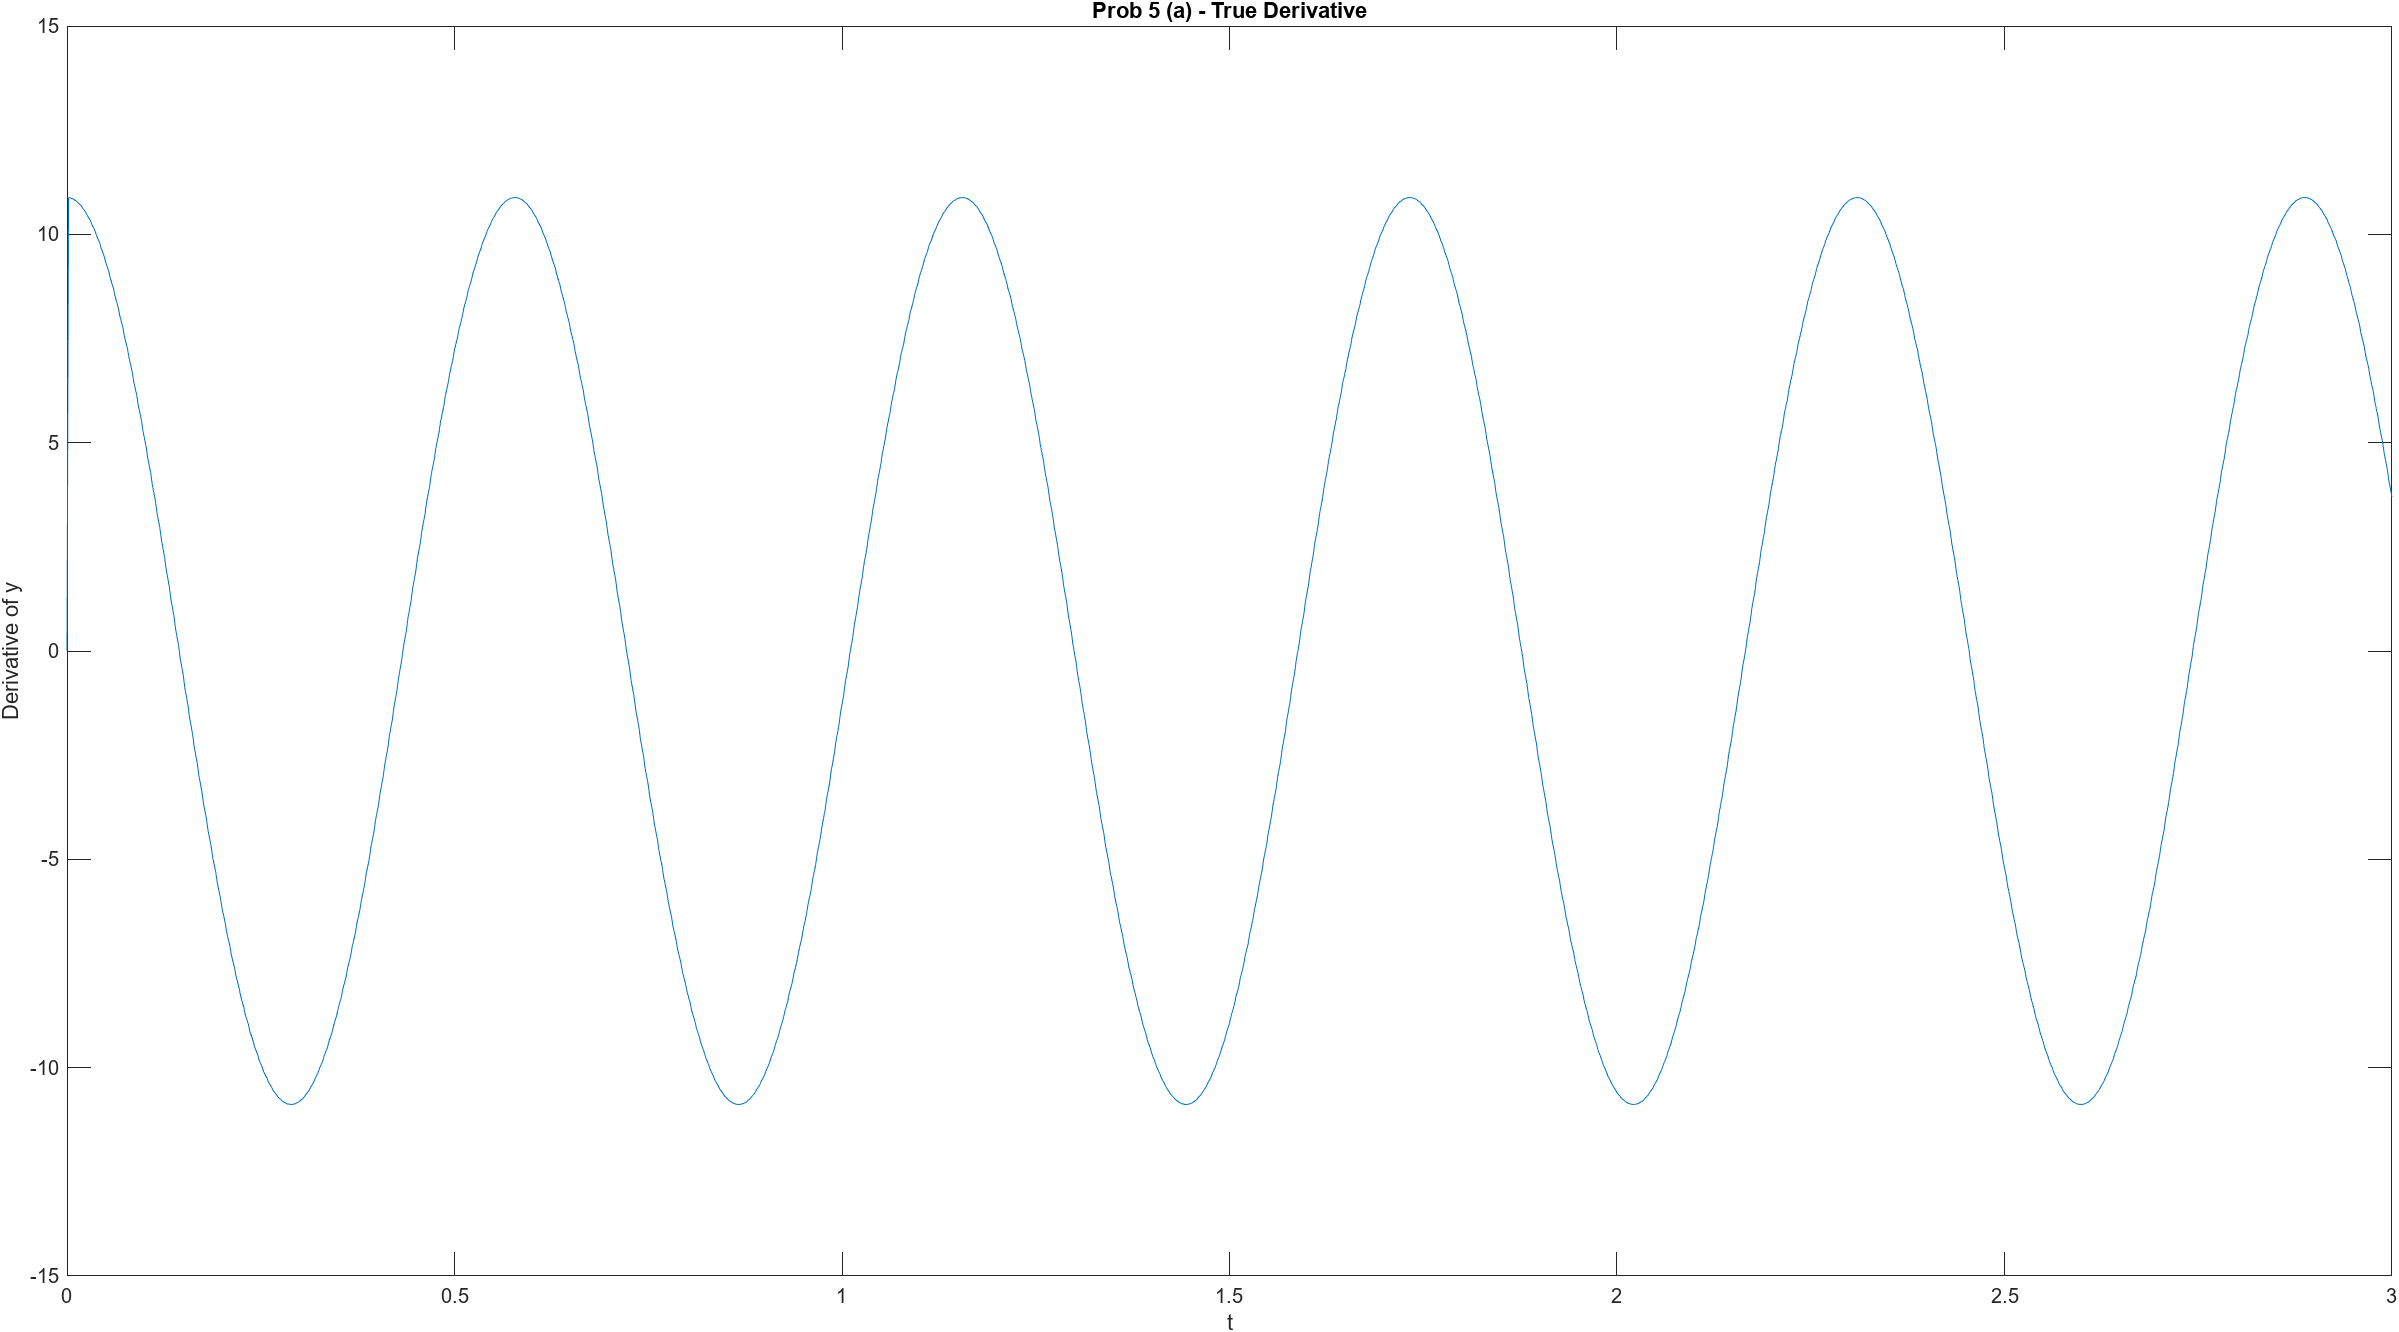
\includegraphics[width=0.75\textwidth]{q5_a_1.png}}
				\caption{True Derivative} 
				\label{fig:q5_a_1}
				\vspace{0.5cm}
			\end{figure}
			Given below is a plot of the naive derivative - 
			\begin{figure}[H]			
				\vspace{0.5cm}
				\centering
				\fbox{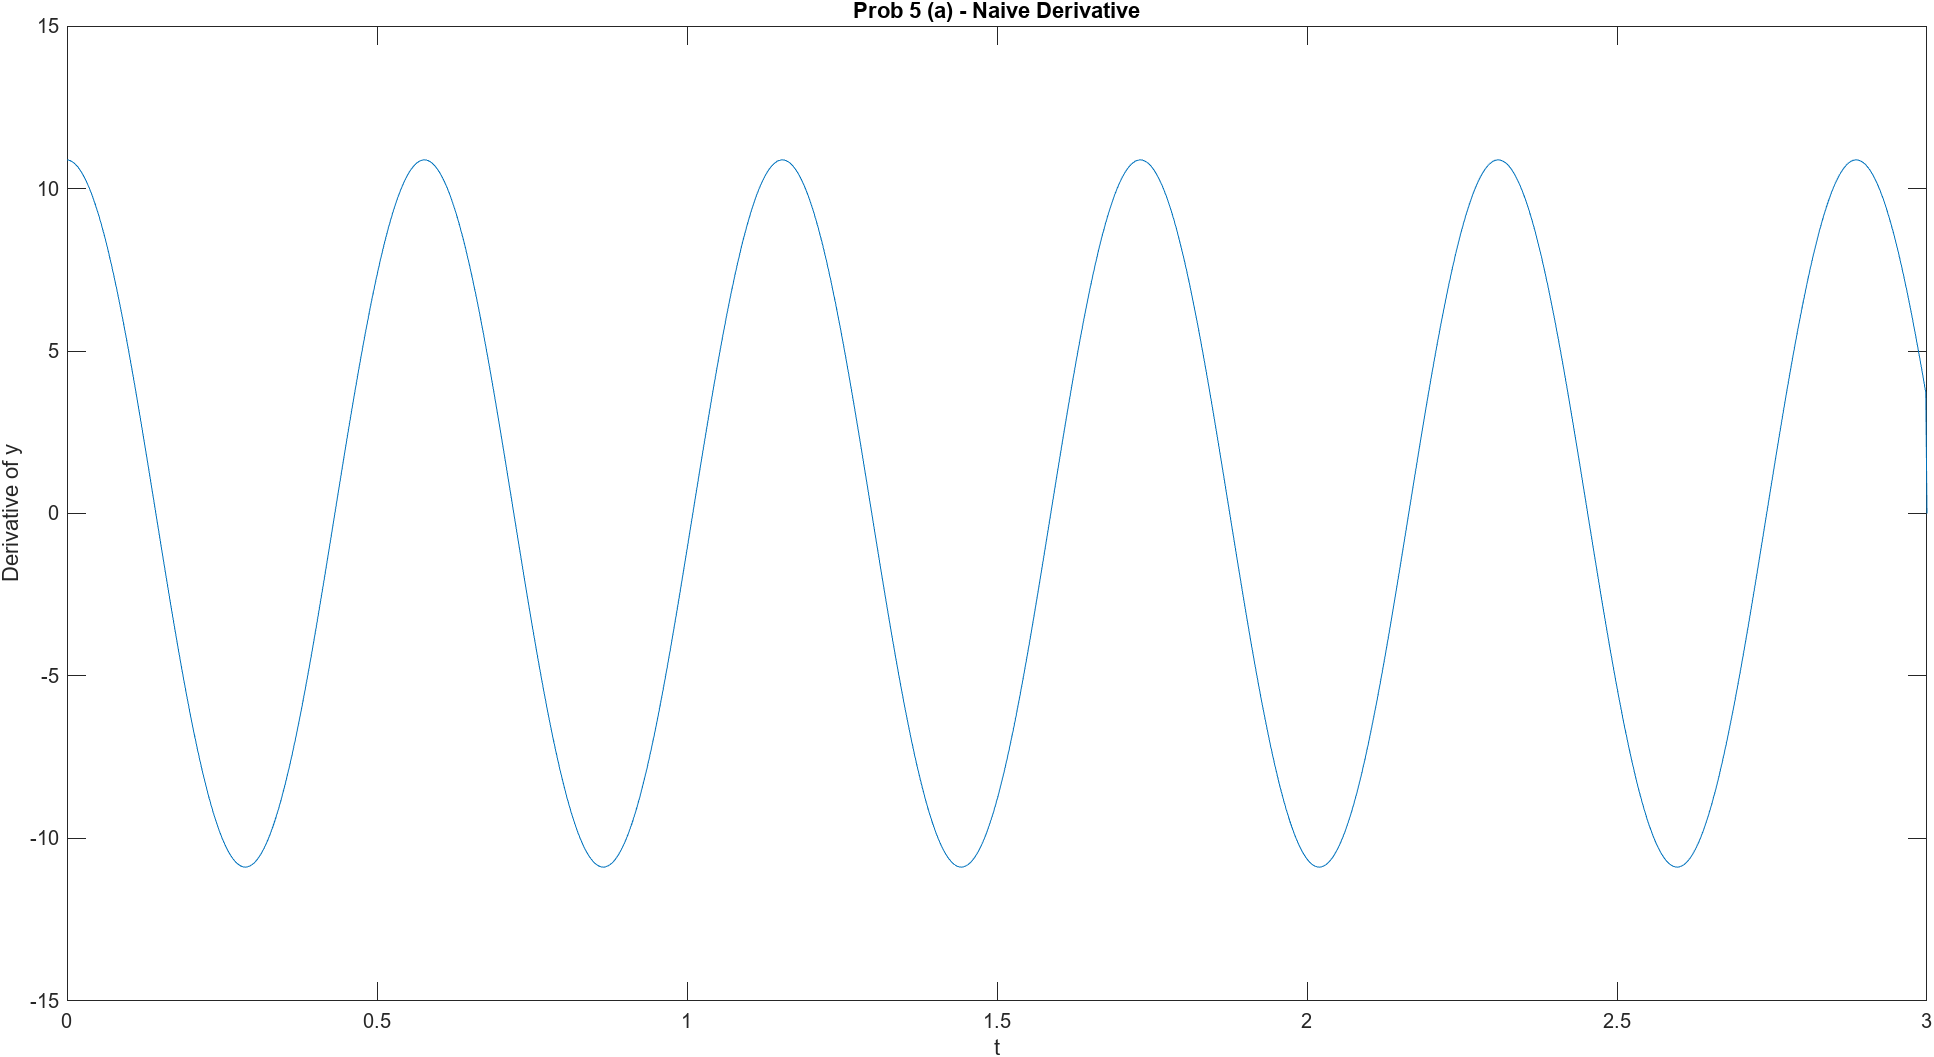
\includegraphics[width=0.75\textwidth]{q5_a_2.png}}
				\caption{Naive Derivative} 
				\label{fig:q5_a_2}
				\vspace{0.5cm}
			\end{figure}
			Given below is a plot of the true and naive derivative. As we can see that they are almost the same, with a very small and negligible difference, which is why they are appear to be nearly coincident.
			\begin{figure}[H]			
				\vspace{0.5cm}
				\centering
				\fbox{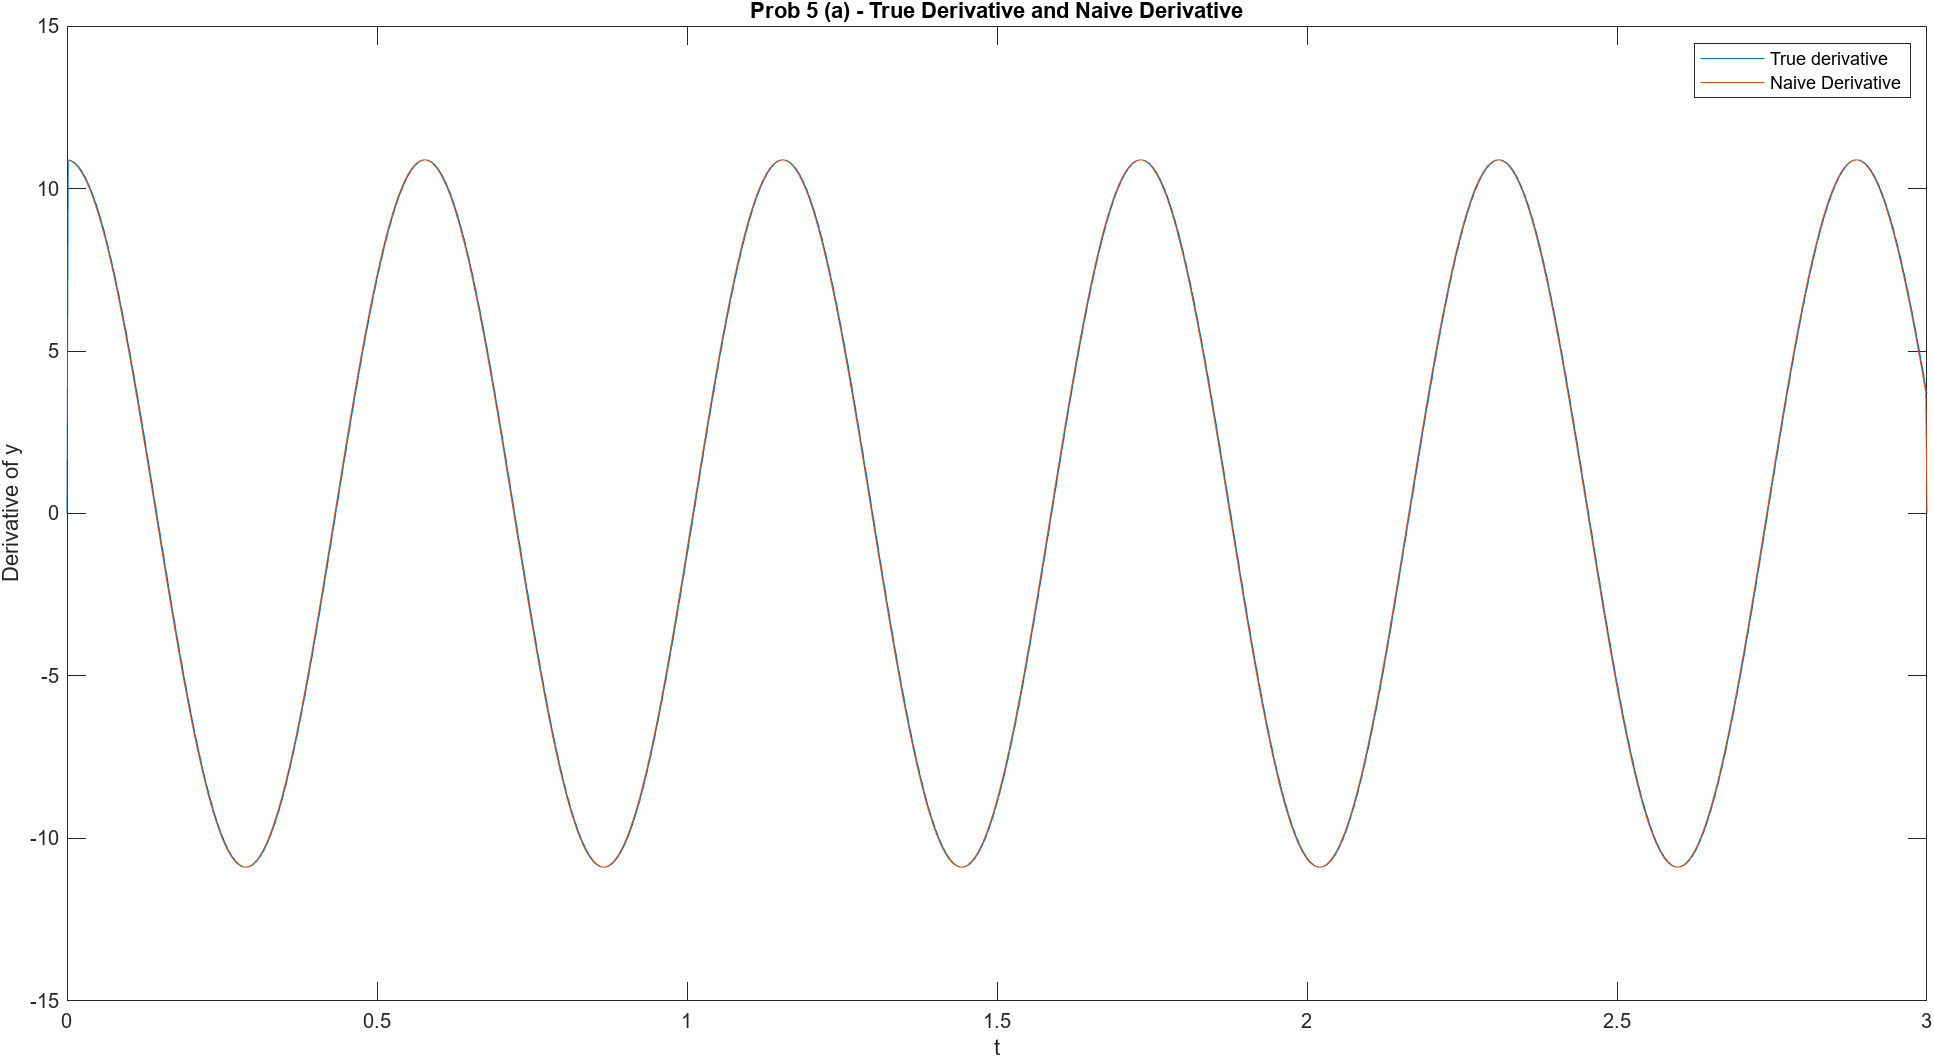
\includegraphics[width=0.75\textwidth]{q5_a_3.png}}
				\caption{True Derivative and Naive Derivative compared} 
				\label{fig:q5_a_3}
				\vspace{0.5cm}
			\end{figure}
			
		\item[Question: 5.(b)] \setcounter{equation}{0}
		\item[Answer:] 	
		
		\item[Question: 6.(a)] \setcounter{equation}{0}
		\item[Answer:] 	Given below is a plot of the true derivative - 
			\begin{figure}[H]			
				\vspace{0.5cm}
				\centering
				\fbox{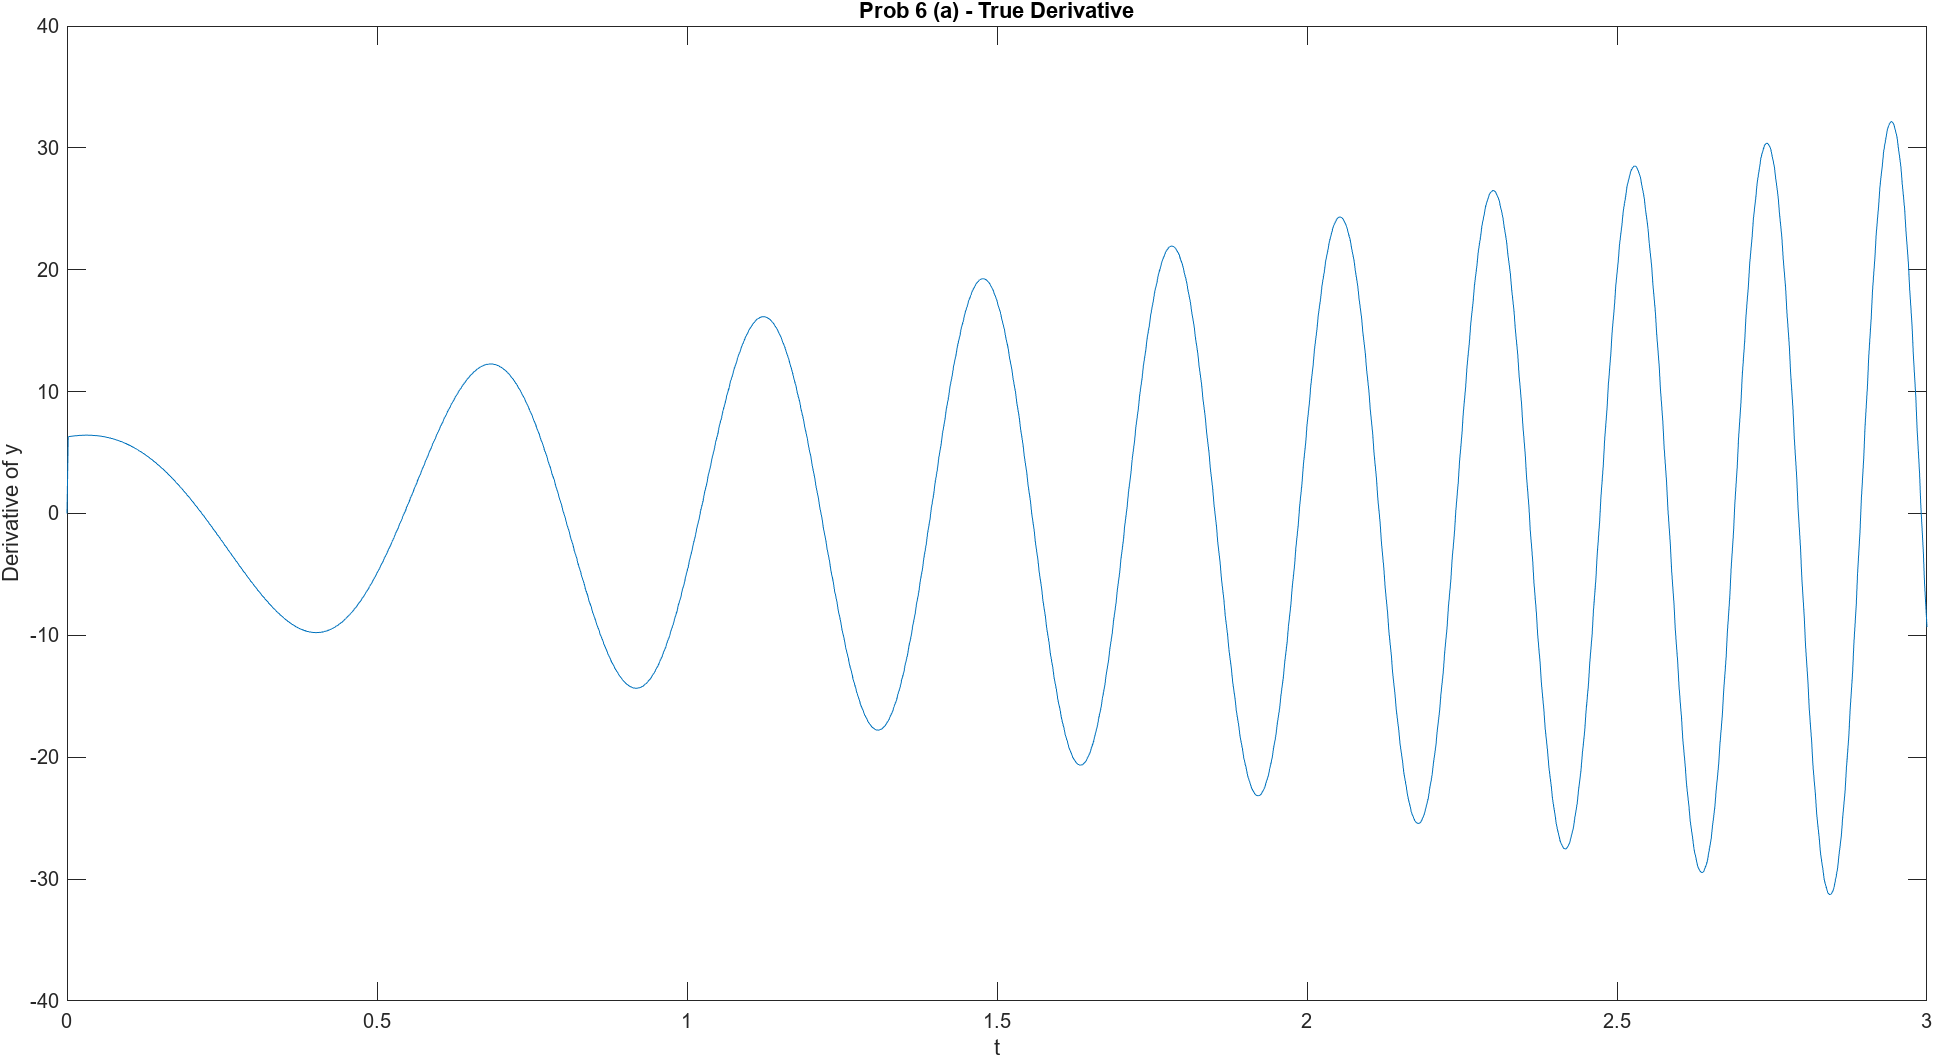
\includegraphics[width=0.75\textwidth]{q6_a_1.png}}
				\caption{True Derivative} 
				\label{fig:q6_a_1}
				\vspace{0.5cm}
			\end{figure}
			Given below is a plot of the naive derivative - 
			\begin{figure}[H]			
				\vspace{0.5cm}
				\centering
				\fbox{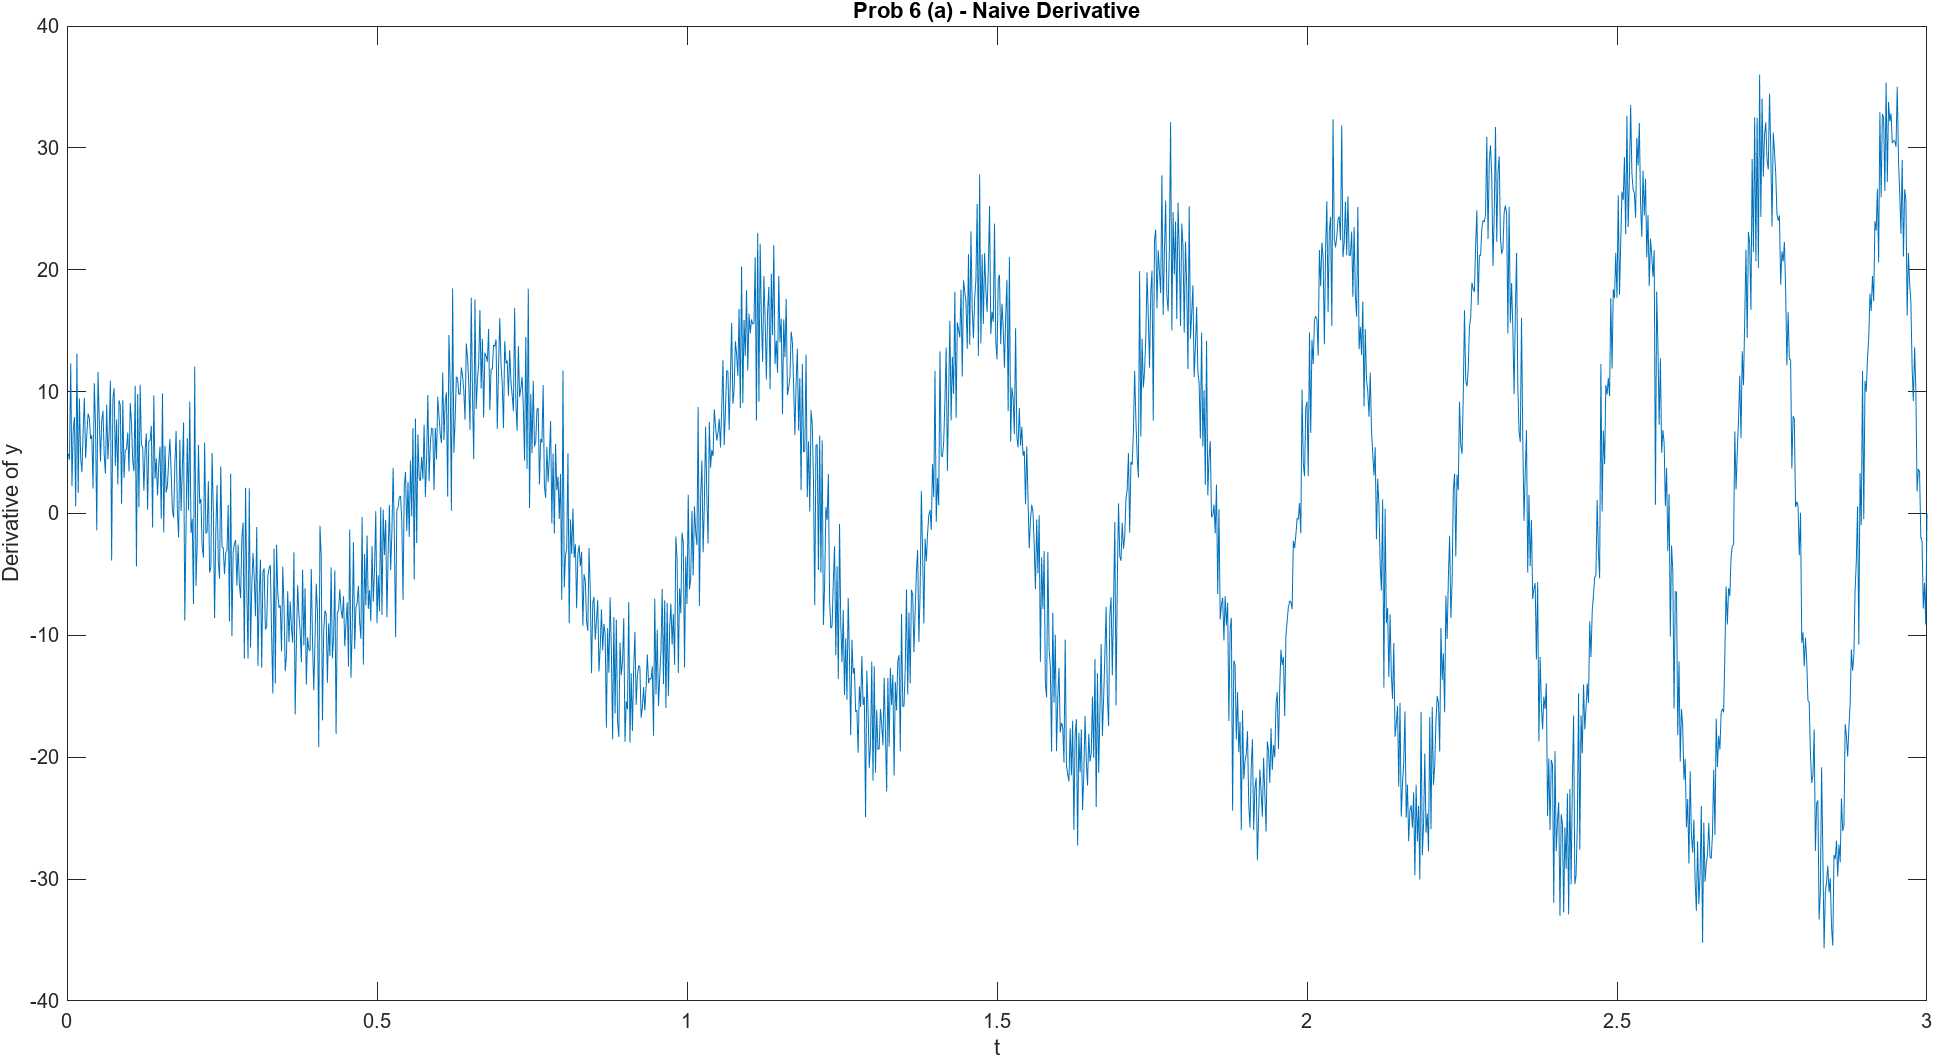
\includegraphics[width=0.75\textwidth]{q6_a_2.png}}
				\caption{Naive Derivative} 
				\label{fig:q6_a_2}
				\vspace{0.5cm}
			\end{figure}
			Given below is a plot of the true and naive derivative. The noise in the system has hidden the true derivative.
			\begin{figure}[H]			
				\vspace{0.5cm}
				\centering
				\fbox{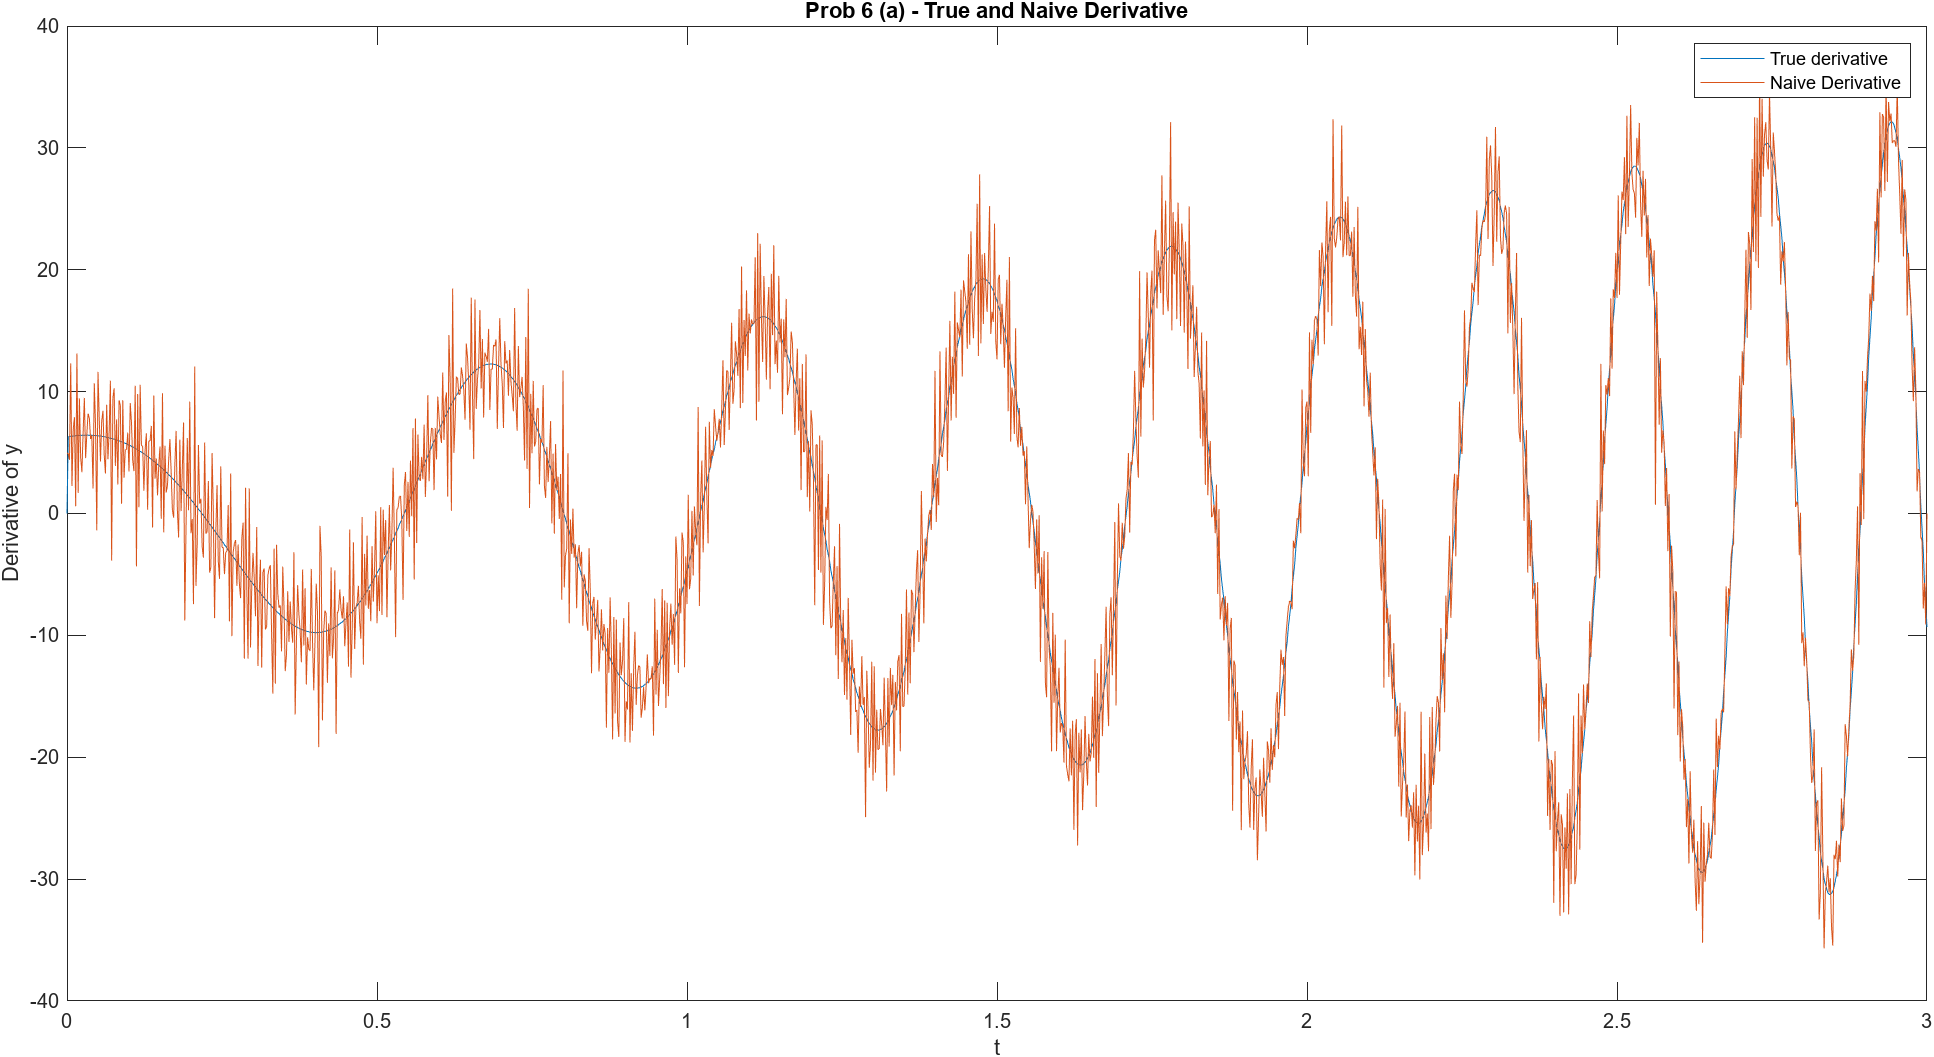
\includegraphics[width=0.75\textwidth]{q6_a_3.png}}
				\caption{True Derivative and Naive Derivative compared} 
				\label{fig:q6_a_3}
				\vspace{0.5cm}
			\end{figure}
		\item[Question: 6.(b)] \setcounter{equation}{0}
		\item[Answer:] 	
		\item[Question: 8.] \setcounter{equation}{0} %A norm $||\cdot||$ on a vector space $(\mathcal{X}, \mathbb{R})$ is said to be strict when $||x+y|| = ||x|| + ||y||$ holds if and only if there exists a non-negative constant $\alpha$ such that either $y = \alpha x$ or $x = \alpha y$. One then says that $(\mathcal{X}, \mathbb{R}, ||\cdot||)$ is strictly normed. Suppose that $(\mathcal{X}, \mathbb{R}, ||\cdot||)$ is strictly normed. Let $M$ be a subspace of $\mathcal{X}$ and suppose that $x \in \mathcal{X}$ is such that $d(x,M) > 0$. Show that there exists ${m}^{*} \in M$ such that \[||x - {m}^{*}|| = d(x,M) := \text{inf}_{y\in M} ||x-y||\] then ${m}^{*}$ is unique.
		\item[Answer:] 	Suppose there exist ${m}_{1},\; {m}_{2} \in M$ and satisfy $||x-{m}_{i}|| = d(x,M)$.
		
		Let $\gamma = d(x,m) \Rightarrow$
		\begin{align}
			\gamma &= \inf_{y\in M} ||x-y|| \leq  ||x - \frac{{m}_{1} + {m}_{2}}{2}|| \\
			&=||\frac{x-{m}_{1}}{2}+\frac{x-{m}_{2}}{2}|| \\
			\text{By given definition of strict norm,} \notag \\
			||\frac{x-{m}_{1}}{2}+\frac{x-{m}_{2}}{2}|| &= \frac{1}{2} ||x-{m}_{1}|| + \frac{1}{2} ||x-{m}_{2}|| \\
			\text{But above ${Eq}^{n}$ would be possible only if} \notag \\
			 \frac{1}{2} ||x-{m}_{1}|| &= \frac{1}{2} ||x-{m}_{2}|| \\
			 \Rightarrow {m}_{1} = {m}_{2}
		\end{align}
		
		$\therefore {m}^{*}$ is unique. \textbf{Q.E.D.}
		
		
		
		
		\item[Question: 9.(a)] \setcounter{equation}{0}
		\item[Answer:] 	Given ${||x||}_{1} = |{x}_{1}| +|{x}_{2}|$. Let $x = \begin{bmatrix}2 \\ 3\end{bmatrix}$ and $y=\begin{bmatrix}4 \\ 5\end{bmatrix}$.
			First let us find ${||x+y||}_{1} \rightarrow$
			\begin{align}
				x+y &= \begin{bmatrix}2+4 \\ 3+5\end{bmatrix} = \begin{bmatrix}6 \\ 8\end{bmatrix} \\
				{||x+y||}_{1} &= |6| + |8| = 14 \label{eq:q9alhs}
			\end{align}
			Now let us find ${||x||}_{1} + {||y||}_{1} \rightarrow$
			\begin{align}
				{||x||}_{1} &= |2| + |3| = 5 \\
				{||y||}_{1} &= |4| + |5| = 9\\
				{||x||}_{1} + {||y||}_{1} &= 5 + 9 = 14 \label{eq:q9arhs}
			\end{align}
			From ${Eq}^{n}(\ref{eq:q9alhs}) = {Eq}^{n}(\ref{eq:q9arhs})$ and the non-existance of an $\alpha$ s.t. $y=\alpha x$ or $x = \alpha y $, we can say that ${||x||}_{1}$ is \underline{\emph{not} strictly normed}.
			
		\item[Question: 9.(c)] \setcounter{equation}{0} 
		\item[Answer:] 	Given ${||x||}_{\infty} = max\{{x}_{1},{x}_{2}\}$. Let $x = \begin{bmatrix}2 \\ 3\end{bmatrix}$ and $y=\begin{bmatrix}4 \\ 5\end{bmatrix}$.
			First let us find ${||x+y||}_{\infty} \rightarrow$
			\begin{align}
				x+y &= \begin{bmatrix}2+4 \\ 3+5\end{bmatrix} = \begin{bmatrix}6 \\ 8\end{bmatrix} \\
				{||x+y||}_{\infty} &= max\{|6|,|8|\} = 8\label{eq:q9clhs}
			\end{align}
			Now let us find ${||x||}_{\infty} + {||y||}_{\infty} \rightarrow$
			\begin{align}
				{||x||}_{\infty} &= max\{|2|,|3|\} = 3 \\
				{||y||}_{\infty} &= max\{|4|,|5|\} = 5 \\
				{||x||}_{\infty} + {||y||}_{\infty} &= 3+5 = 8 \label{eq:q9crhs}
			\end{align}
			From ${Eq}^{n}(\ref{eq:q9clhs}) = {Eq}^{n}(\ref{eq:q9crhs})$ and the non-existance of an $\alpha$ s.t. $y=\alpha x$ or $x = \alpha y $, we can say that ${||x||}_{\infty}$ is \underline{\emph{not} strictly normed}.
	\end{qalist}
\end{document}